\begin{frame}{Core - Selection criteria}
  \begin{itemize}
    \item Multicore capable design.
    \item Linux bootable.
    \item Open/accessible design.
    \item Fit resource constraints of our fpga. 
    \item Maximize compatibility with our fpga.
  \end{itemize}
\end{frame}

\begin{frame}{Core - First try: Ariane}
\begin{columns}[T]
  \begin{column}{0.5\textwidth} % Left column and width

\begin{itemize}
    \item Ariane is a 6-stage in-order CPU
    \item Implements privilege levels M, S, U to fully support a Unix-like operating system
    \item 
\end{itemize}
\end{column}
\begin{column}{.5\textwidth} % Right column and width

\begin{figure}[!ht]
    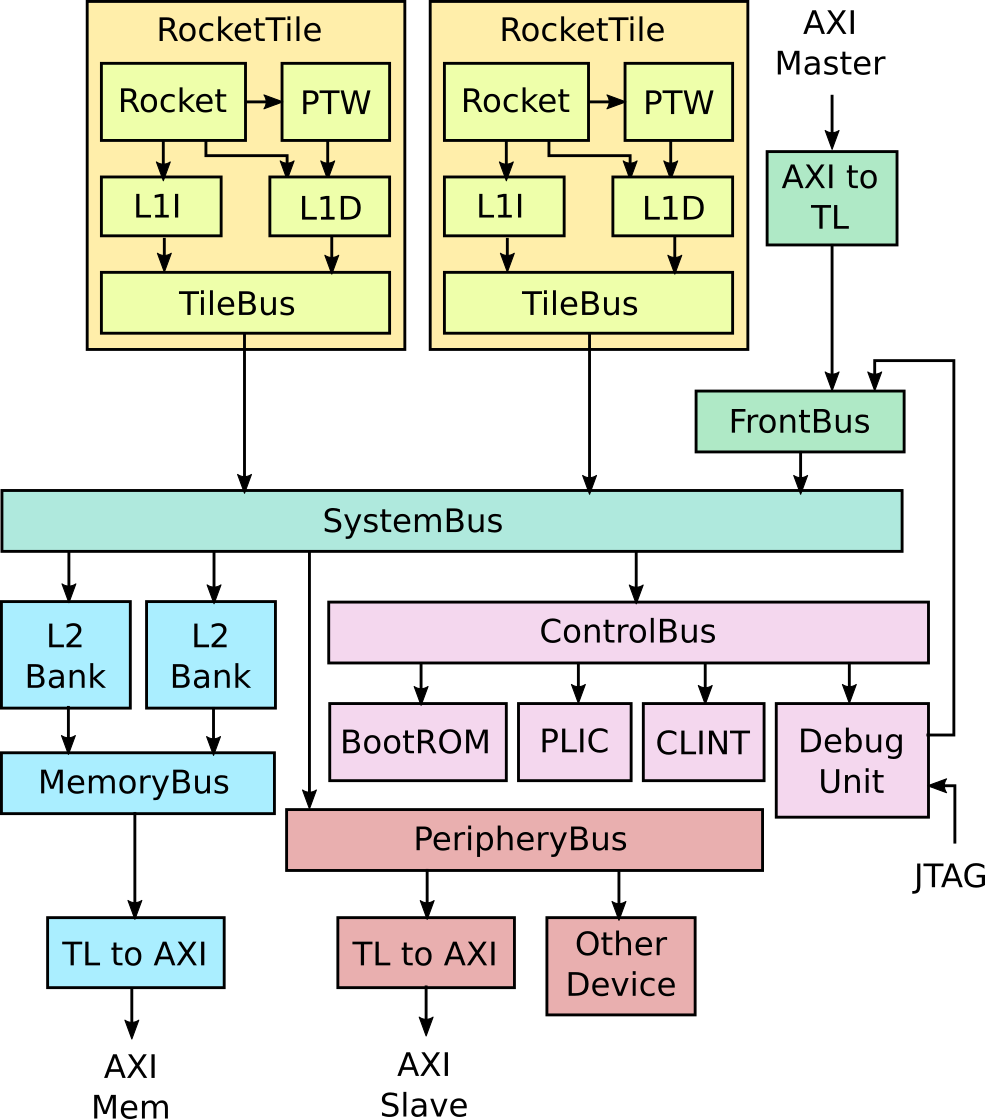
\includegraphics[width=1\linewidth]{images/rocketchip-diagram.png}
\end{figure}
\end{column}
\end{columns}
\end{frame}

\begin{frame}{Core - First try: Ariane}
    \begin{itemize}
            \item Boots Linux.
            \item Multi-Core capable.
            \item Open design.
    \end{itemize}

    \begin{alertblock}{Issue}
            Too complex and too much effort to port the design to be compatible with our FPGA.	
    \end{alertblock}
\end{frame}



\begin{frame}{RISC-V: Rocket Chip}
\begin{columns}[T]
  \begin{column}{0.5\textwidth} % Left column and width
Rocket Chip is a SoC generator for Rocket Cores
\begin{itemize}
    \item Developed in Berkley, EEUU
    \item Hardware generation is done using Chisel
    \item Rocket core: 
    \begin{itemize}
        \item In-order scalar processor with 5-stage pipeline
        \item RV64G variant of the RISC-V ISA
    \end{itemize}
\end{itemize}
\end{column}
\begin{column}{.5\textwidth} % Right column and width

\begin{figure}[!ht]
    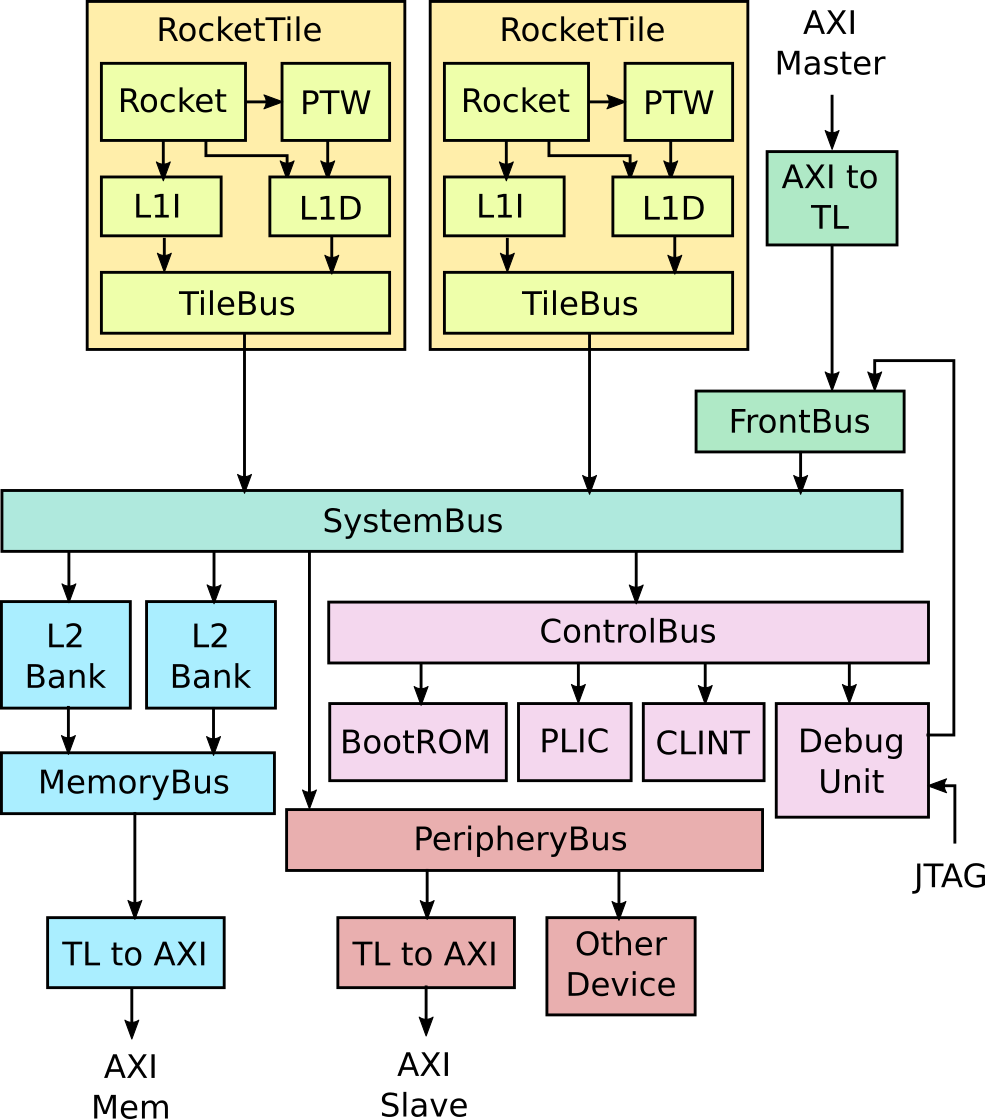
\includegraphics[width=1\linewidth]{images/rocketchip-diagram.png}
\end{figure}
\end{column}
\end{columns}
\end{frame}

\begin{frame}{Core - Second try: Rocket Chip}
  \begin{itemize}
    \item \gls{soc} generator based on Rocket scalar cores.
    \item Multi-core system capable with option to add coherent memory systems.
    \item Boots Linux.
    \item Open source.
  \end{itemize}

  \begin{alertblock}{Issue}
    Scala based configuration. Lack of documentation. Not clear on how to generate a bitstream for our \gls{fpga}.
  \end{alertblock}
\end{frame}


\begin{frame}{Core - Final selection: Darkriscv}
  \begin{itemize}
    \item Low resource utilisation.
    \item Simple design. Implements 
  \end{itemize}
\end{frame}